\documentclass[aspectratio=169,11pt]{beamer}

\usetheme{Madrid}
\setbeamertemplate{navigation symbols}{}
\setbeamertemplate{caption}[numbered]

\usepackage[T1]{fontenc}
\usepackage[utf8]{inputenc}
\usepackage[polish]{babel}
\usepackage{lmodern}
\usepackage{graphicx}
\usepackage{booktabs}
\usepackage{array}
\usepackage{makecell}
\usepackage{xcolor}
\usepackage{tikz}
\usetikzlibrary{arrows.meta,positioning,shapes.geometric,calc,fit,backgrounds}

% --- wspólne style diagramów --------------------------------------------------
\tikzset{
  box/.style   = {rectangle, rounded corners=2pt, draw=black!70, thick,
                  fill=blue!8, align=center, minimum height=8mm, inner sep=4pt,
                  font=\scriptsize},
  hot/.style   = {box, fill=orange!18, draw=orange!70!black},
  fb/.style    = {box, fill=green!10, draw=good!80!black},
  isle/.style  = {circle, draw=black!70, thick, fill=blue!10, align=center,
                  minimum size=10mm, font=\tiny},
  cell/.style  = {rectangle, draw=black!45, fill=orange!12, minimum size=3.4mm,
                  inner sep=0pt},
  fl/.style    = {-{Stealth[length=2mm]}, thick},
  flb/.style   = {{Stealth[length=2mm]}-{Stealth[length=2mm]}, thick},
  dashfl/.style  = {fl, densely dashed, draw=good!70!black},
}

% szuka wykresów w katalogu głównym, w figures/ oraz w lokalizacji oryginalnej
\graphicspath{{./}{figures/}{../results/plots/}}

% --- skróty kolorystyczne -----------------------------------------------------
\definecolor{good}{RGB}{30,130,60}
\definecolor{bad}{RGB}{190,40,40}
\newcommand{\good}[1]{\textcolor{good}{\textbf{#1}}}
\newcommand{\bad}[1]{\textcolor{bad}{\textbf{#1}}}

\title[Zrównoleglenie HGS-CVRP]{Zrównoleglenie algorytmu HGS dla problemu CVRP}
\subtitle{Analiza wpływu GPU, modelu master--slave i modelu wysp na jakość rozwiązań}
\author{Hubert Blonowski, Jan Zaborski}
\date{14 czerwca 2026}

\begin{document}

% ---------------------------------------------------------------------------
\begin{frame}
  \titlepage
\end{frame}

\begin{frame}{Plan prezentacji}
  \tableofcontents
\end{frame}

% ===========================================================================
\section{Problem CVRP}
% ===========================================================================
\begin{frame}{Czym jest CVRP?}
  \textbf{Capacitated Vehicle Routing Problem} — kanoniczny problem optymalizacji tras.
  \vfill
  \begin{columns}[T]
    \begin{column}{0.58\textwidth}
      Dane:
      \begin{itemize}
        \item jeden magazyn (depot) i $n$ klientów,
        \item każdy klient ma zapotrzebowanie $q_i$,
        \item flota pojazdów o jednakowej pojemności $Q$,
        \item macierz odległości (kosztów) między punktami.
      \end{itemize}
      \vspace{0.4em}
      Cel: znaleźć zbiór tras (każda zaczyna i kończy się w depot) o \textbf{minimalnej łącznej długości}, tak aby:
      \begin{itemize}
        \item każdy klient był odwiedzony dokładnie raz,
        \item suma zapotrzebowań na trasie $\le Q$.
      \end{itemize}
    \end{column}
    \begin{column}{0.42\textwidth}
      \centering
      \begin{tikzpicture}[scale=0.9]
        \node[rectangle,draw,fill=blue!20] (d) at (0,0) {Depot};
        \foreach \x/\y in {-1.4/1.2, -1.6/-0.6, 1.3/1.3, 1.7/0.1, 1.2/-1.2, -0.3/-1.5}
          \fill[black] (\x,\y) circle (2pt);
        \draw[good,thick] (d) -- (-1.4,1.2) -- (-1.6,-0.6) -- (d);
        \draw[bad,thick] (d) -- (1.3,1.3) -- (1.7,0.1) -- (d);
        \draw[orange,thick] (d) -- (1.2,-1.2) -- (-0.3,-1.5) -- (d);
      \end{tikzpicture}
    \end{column}
  \end{columns}
\end{frame}

\begin{frame}{Dlaczego to trudny problem?}
  \begin{itemize}
    \item CVRP jest \textbf{NP-trudny} — uogólnia problem komiwojażera (TSP).
    \item Przestrzeń rozwiązań rośnie wykładniczo wraz z liczbą klientów.
    \item Dla instancji z tysiącami klientów dokładne metody są bezużyteczne — stosuje się \textbf{metaheurystyki}.
    \item Praktyczne znaczenie: logistyka, kurierzy, dystrybucja, zbiórka odpadów — drobna poprawa \% tras = realne oszczędności paliwa i czasu.
  \end{itemize}
  \vfill
  \begin{block}{State of the art}
    \textbf{HGS} (Hybrid Genetic Search) Vidala i in. jest jednym z najlepszych znanych algorytmów dla CVRP — bardzo dobre rozwiązania w krótkim czasie.
  \end{block}
\end{frame}

% ===========================================================================
\section{Algorytm HGS}
% ===========================================================================
\begin{frame}{Główna idea: ,,hodujemy'' rozwiązania jak w ewolucji}
  Nie da się sprawdzić wszystkich możliwych zestawów tras — jest ich astronomicznie wiele. Zamiast tego \textbf{naśladujemy dobór naturalny}:
  \vfill
  \begin{enumerate}
    \item Trzymamy \textbf{zbiór gotowych rozwiązań} (każde to kompletny plan tras).
    \item Bierzemy dwa dobre rozwiązania i \textbf{,,krzyżujemy'' je} — powstaje nowe, dziedziczące fragmenty po obojgu ,,rodzicach''.
    \item Nowe rozwiązanie \textbf{podszlifowujemy} drobnymi poprawkami (przeszukiwanie lokalne).
    \item Najlepsze przeżywają, słabe odrzucamy. \textbf{Powtarzamy tysiące razy.}
  \end{enumerate}
\end{frame}

\begin{frame}{Jak wygląda jedna ,,tura'' algorytmu}
  \centering
  \begin{tikzpicture}[node distance=6mm and 9mm]
    \node[box] (pop)  {Populacja\\\scriptsize(zbiór rozwiązań)};
    \node[box, right=of pop] (cx) {Krzyżowanie\\\scriptsize(2 rodziców\\$\rightarrow$ potomek)};
    \node[box, right=of cx]  (sp) {Split\\\scriptsize(podział\\na trasy)};
    \node[hot, right=of sp]  (ls) {Przeszukiwanie\\lokalne\\\scriptsize(,,szlif'')};
    \node[box, right=of ls]  (ins){Dodaj do populacji,\\odrzuć najsłabsze};
    % główny przepływ
    \draw[fl] (pop)--(cx);
    \draw[fl] (cx)--(sp);
    \draw[fl] (sp)--(ls);
    \draw[fl] (ls)--(ins);
    % pętla powrotna
    \draw[fl] (ins.north) .. controls +(0,1.1) and +(0,1.1) .. node[above,font=\scriptsize]{kolejna tura} (pop.north);
    % blok sprzężenia
    \node[fb, below=14mm of sp] (fbk) {Bieżące ,,reguły gry'':\\\textbf{kary} za przeładowanie + dbanie o \textbf{różnorodność}};
    \draw[dashfl] (fbk) -- (ls);
    \draw[dashfl] (fbk.west) -| (pop.south);
    \draw[dashfl] (fbk.east) -| (ins.south);
  \end{tikzpicture}
\end{frame}
% ===========================================================================
\section{Wprowadzone modyfikacje}
% ===========================================================================
\begin{frame}{Trzy osie zrównoleglenia}
  Dodaliśmy do HGS trzy niezależne (i łączalne) mechanizmy:
  \vfill
  \begin{columns}[T]
    \begin{column}{0.33\textwidth}
      \begin{block}{1. GPU SWAP* (CUDA)}
        Ewaluacja par klientów dla SWAP* przeniesiona na GPU. Tysiące par liczonych równolegle, strumienie CUDA.
      \end{block}
    \end{column}
    \begin{column}{0.33\textwidth}
      \begin{block}{2. Master--slave (OpenMP)}
        Równoległe wytwarzanie potomstwa: 16 potomków na rundę, 8 wątków. ,,Many offspring''.
      \end{block}
    \end{column}
    \begin{column}{0.33\textwidth}
      \begin{block}{3. Model wysp (MPI)}
        8 niezależnych populacji (wysp), topologia gwiazdy, polityki migracji i selekcji migrantów.
      \end{block}
    \end{column}
  \end{columns}
  \vfill
  Dodatkowo: warstwa \textbf{telemetrii} i \textbf{monitor sprzętu} (zużycie CPU/GPU) do rzetelnej oceny.
  \vfill
  {\footnotesize Z tych mechanizmów złożyliśmy \textbf{6 wariantów testowych}: \texttt{baseline}, \texttt{gpu}, \texttt{offspring16t8}, \texttt{gpu\_offspring16t8}, \texttt{island8\_star}, \texttt{island8\_star\_gpu\_off16t8}.}
\end{frame}

% ---------------------------------------------------------------------------
%  OŚ 1 — GPU SWAP*
% ---------------------------------------------------------------------------
\begin{frame}{Oś 1: SWAP* na GPU — pomysł}
  \textbf{Co chcemy przyspieszyć?} W każdym ,,szlifie'' rozwiązania algorytm sprawdza \textbf{ogromną liczbę par klientów} z różnych tras: czy ich zamiana skróci trasy? To miliony niezależnych, identycznych obliczeń — \emph{idealne dla GPU}, które liczy tysiące takich par naraz.
  \vfill
  \centering
  \begin{tikzpicture}[node distance=14mm]
    \node[box, fill=blue!12] (host) {\textbf{Host (CPU)}\\\scriptsize pętla przeszukiwania,\\bieżące trasy};
    \node[draw, thick, rounded corners, fill=orange!8, right=34mm of host,
          minimum width=30mm, minimum height=22mm, label={[font=\scriptsize]above:\textbf{GPU} — siatka wątków}] (gpu) {};
    \foreach \r in {0,1,2}\foreach \c in {0,1,2,3,4}
      \node[cell] at ($(gpu.center)+(-1.0+\c*0.5,0.55-\r*0.55)$) {};
    \draw[fl] (host.north east) ++(0,1mm) .. controls +(12mm,7mm) and +(-12mm,7mm) ..
          node[above,font=\tiny]{kopiuj \textbf{pary} klientów} (gpu.north west);
    \draw[fl, draw=good!70!black] (gpu.south west) .. controls +(-12mm,-7mm) and +(12mm,-7mm) ..
          node[below,font=\tiny]{zwróć najlepszą zamianę} (host.south east);
  \end{tikzpicture}
  \vfill
  {\footnotesize Każda komórka GPU ocenia jedną parę klientów; CPU dostaje gotowy ranking najlepszych zamian.}
\end{frame}

\begin{frame}{Oś 1: SWAP* na GPU — co zbudowaliśmy i kompromis}
      \textbf{Co zbudowaliśmy (CUDA)}
      \begin{itemize}
        \item \textbf{kernel} liczący koszt zamiany dla wszystkich par równolegle,
        \item \textbf{spłaszczony układ danych} tras (\texttt{GpuDataLayout}) dla szybkiego dostępu do pamięci GPU,
        \item \textbf{strumienie CUDA} — nakładanie obliczeń i transferów,
        \item pomiar zużycia GPU przez \textbf{NVML}.
      \end{itemize}
\end{frame}

% ---------------------------------------------------------------------------
%  OŚ 2 — master-slave (OpenMP)
% ---------------------------------------------------------------------------
\begin{frame}{Oś 2: model master--slave — pomysł}
  \textbf{Co chcemy przyspieszyć?} Najdroższy krok tury to ,,szlif'' potomka (przeszukiwanie lokalne). Skoro mamy wiele rdzeni CPU — \textbf{wyprodukujmy wielu potomków naraz}, każdy szlifowany na osobnym wątku.
  \vfill
  \centering
  \begin{tikzpicture}[node distance=8mm and 12mm]
    \node[box, fill=blue!12] (m) {\textbf{Master}\\\scriptsize wybiera rodziców,\\rozdziela zadania};
    \node[hot, above right=2mm and 16mm of m] (w1) {Wątek 1\\\scriptsize krzyżowanie + szlif};
    \node[hot, right=16mm of m]               (w2) {Wątek 2\\\scriptsize krzyżowanie + szlif};
    \node[hot, below right=2mm and 16mm of m] (w3) {Wątek $k$\\\scriptsize krzyżowanie + szlif};
    \foreach \w in {w1,w2,w3}{
      \draw[fl] (m.east) -- (\w.west);
      \draw[fl, draw=good!70!black] (\w.west) ++(0,-1mm) .. controls +(-6mm,-4mm) and +(6mm,-4mm) .. (m.east);
    }
  \end{tikzpicture}
  \vfill
  {\footnotesize W naszym wariancie: \textbf{16 potomków na rundę, 8 wątków}.}
\end{frame}

\begin{frame}{Oś 2: model master--slave — co zbudowaliśmy i kompromis}
      \textbf{Co zbudowaliśmy (OpenMP)}
      \begin{itemize}
        \item wspólny interfejs \texttt{OffspringMaker} z dwiema implementacjami: \texttt{Standard} (sekwencyjna) i \texttt{Parallel},
        \item \texttt{ParallelOffspringMaker} — master rozdziela zadania, wątki liczą krzyżowanie + Split + szlif,
        \item sterowanie parametrami: liczba potomków i liczba wątków,
        \item dodatkowo: równoległa ścieżka SWAP* na CPU (\texttt{OpenMPLocalSearch}).
      \end{itemize}
\end{frame}

% ---------------------------------------------------------------------------
%  OŚ 3 — model wysp (MPI)
% ---------------------------------------------------------------------------
\begin{frame}{Oś 3: model wysp — pomysł}
  \textbf{Inne podejście do równoległości:} zamiast jednej populacji uruchamiamy \textbf{kilka niezależnych HGS} (,,wysp'') obok siebie. Co jakiś czas wyspy \textbf{wymieniają się najlepszymi rozwiązaniami} (migracja), by nawzajem się inspirować.
  \vfill
  \centering
  \begin{tikzpicture}
    \node[isle, fill=blue!18] (hub) at (0,0) {Hub};
    \foreach \i/\a in {1/30,2/77,3/124,4/171,5/218,6/265,7/312}{
      \node[isle] (i\i) at (\a:1.9) {HGS\\\i};
      \draw[flb, draw=good!60!black] (hub) -- (i\i);
    }
  \end{tikzpicture}
  \vfill
  {\footnotesize Topologia \textbf{gwiazdy}: 8 wysp wymienia migrantów przez centralny węzeł. Każda wyspa = \textbf{pełny HGS} na własnej podpopulacji.}
\end{frame}

\begin{frame}{Oś 3: model wysp — co zbudowaliśmy i kompromis}
      \textbf{Co zbudowaliśmy (MPI, modularnie)}
      \begin{itemize}
        \item wymienne \textbf{topologie} połączeń (m.in.\ gwiazda),
        \item \textbf{polityki migracji} — kiedy i jak często wysyłać,
        \item \textbf{selektory migrantów} — kogo wysłać (np.\ najlepszego),
        \item obsługa imigrantów i \textbf{komunikator} (synchroniczny, MPI).
      \end{itemize}
\end{frame}


% ===========================================================================
\section{Wyniki eksperymentów}
% ===========================================================================
\begin{frame}{Konfiguracja eksperymentów}
  \begin{itemize}
    \item \textbf{5 instancji XL} (2354–10001 klientów), \textbf{6 wariantów}, \textbf{limit czasu 600 s}, seed 1.
    \item Mierzone: jakość (koszt), liczba tur algorytmu, ewaluowane pary SWAP*, ruchy lokalne, wykorzystanie CPU/GPU, migracje, rundy potomstwa.
  \end{itemize}
\end{frame}

\begin{frame}{Poprawa jakości względem baseline}
  \centering
  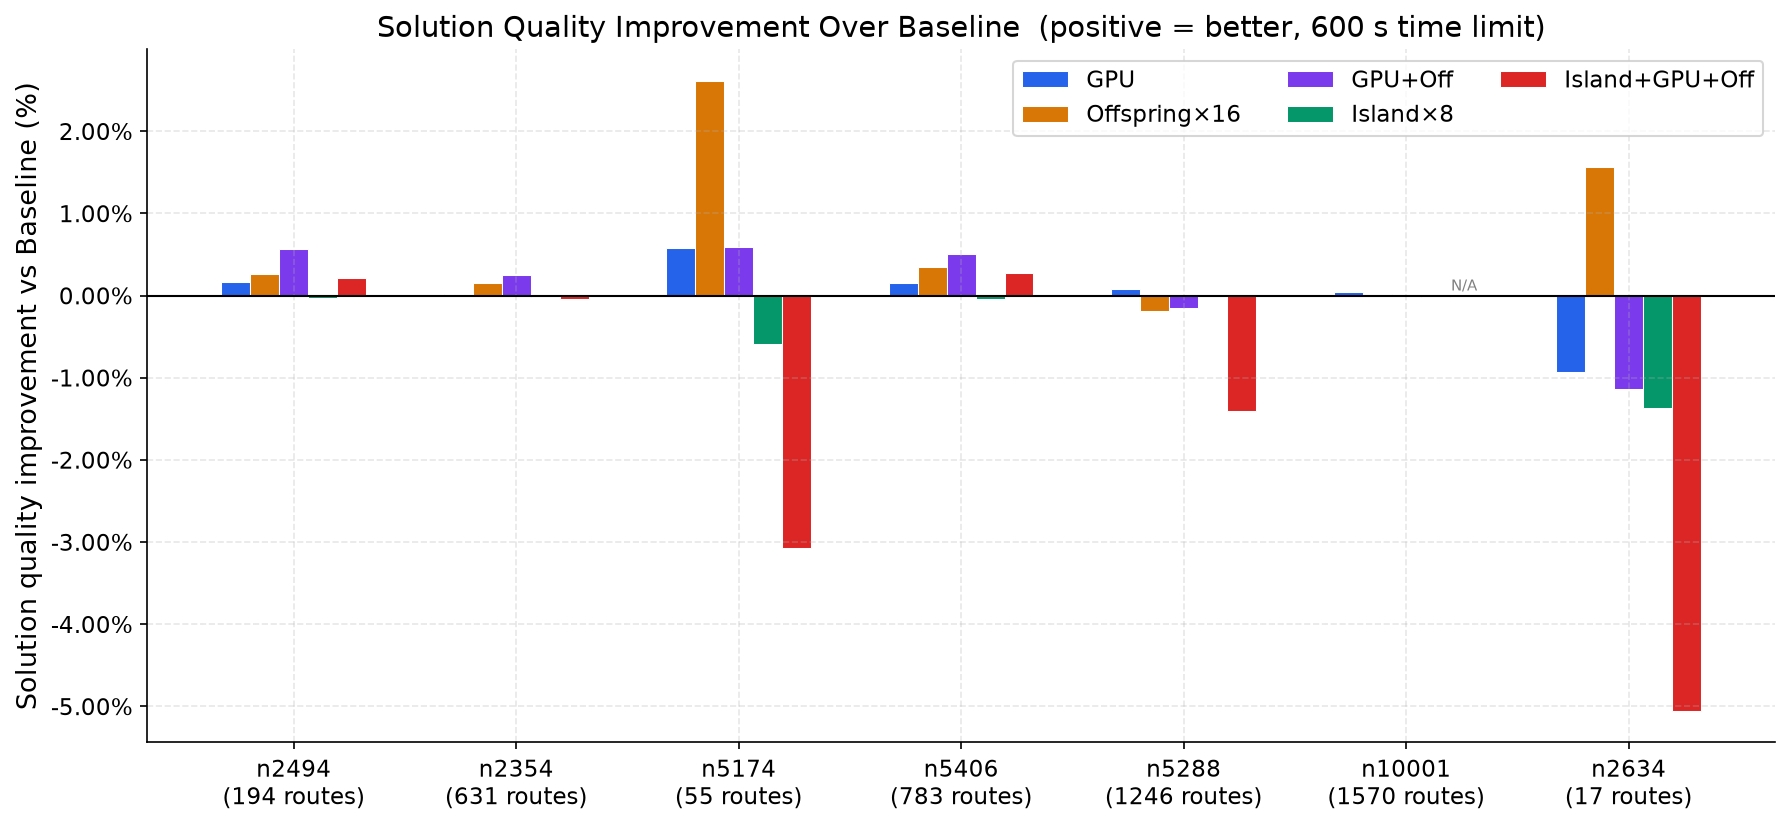
\includegraphics[height=0.78\textheight]{01_quality_improvement.png}
  \par\footnotesize Wartość dodatnia = lepiej niż baseline. Skala efektu: ułamki procenta.
\end{frame}

\begin{frame}{Mapa cieplna jakości — gdzie jest zielono, a gdzie czerwono}
  \centering
  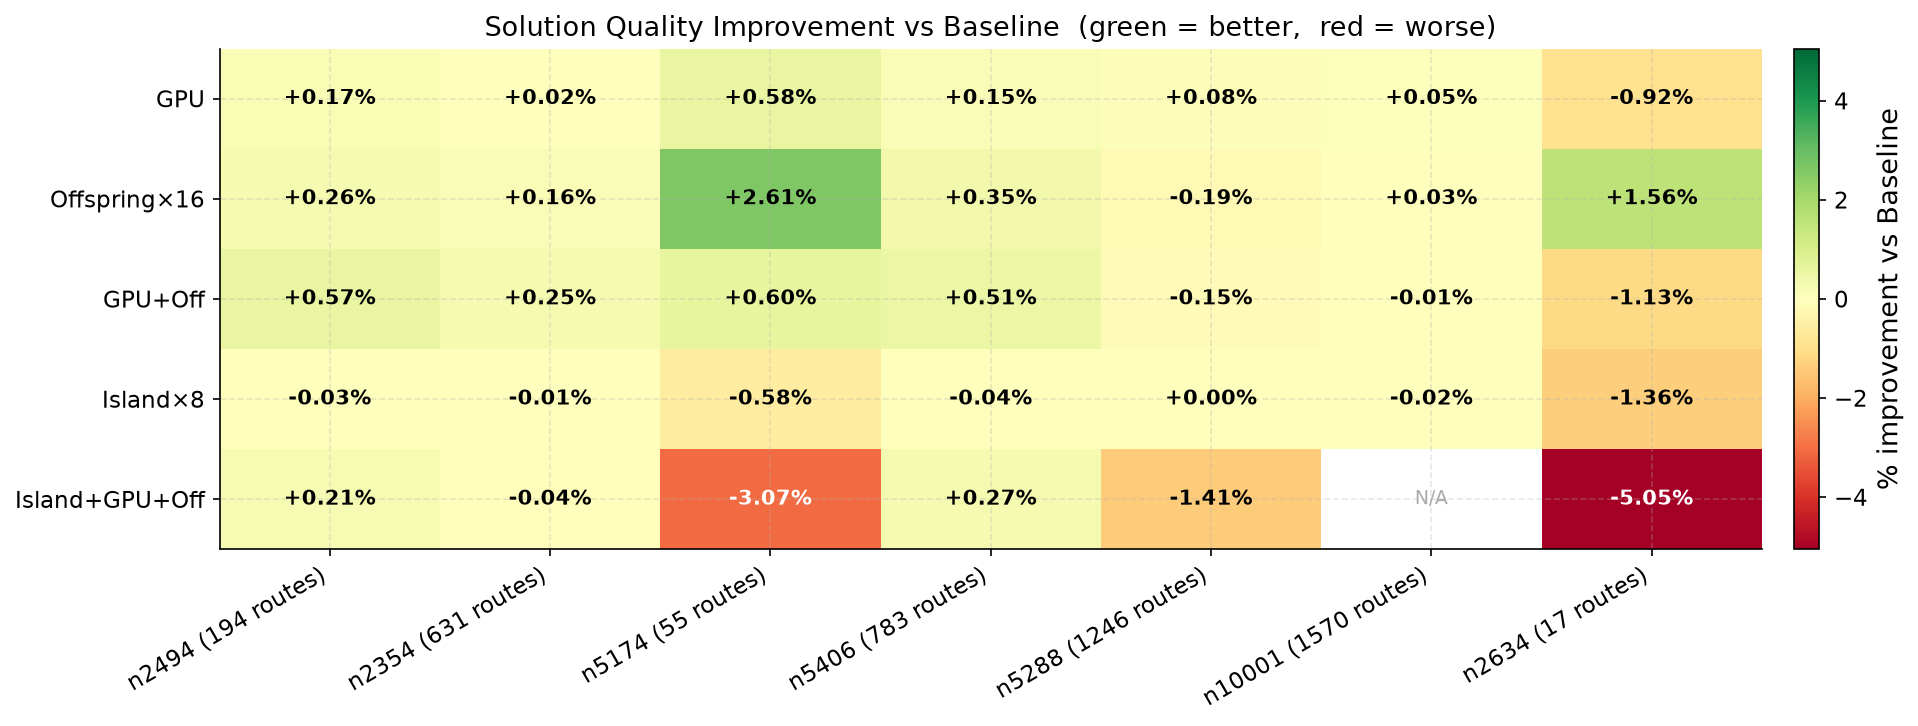
\includegraphics[width=\textwidth,height=0.74\textheight,keepaspectratio]{07_quality_heatmap.png}
  \par\medskip\begin{minipage}{0.92\textwidth}\footnotesize Najbardziej złożony wariant (wyspy+GPU+offspring) jest często \bad{czerwony} — gorszy od baseline.\end{minipage}
\end{frame}


\begin{frame}{Liczby — najlepszy wariant na każdej instancji}
  \centering
  \small
  \begin{tabular}{l r r r l}
    \toprule
    Instancja & Baseline & Najlepszy wariant & $\Delta$ & Który wariant \\
    \midrule
    XL-n2354-k631  & 947\,790   & 945\,389   & \good{+0,25\%} & GPU+Off \\
    XL-n2494-k194  & 366\,131   & 364\,057   & \good{+0,57\%} & GPU+Off \\
    XL-n2634-k17   & 33\,220    & 32\,701    & \good{+1,56\%} & Offspring \\
    XL-n5174-k55   & 65\,467    & 63\,756    & \good{+2,61\%} & Offspring \\
    XL-n5288-k1246 & 1\,984\,069 & 1\,982\,432 & \good{+0,08\%} & GPU \\
    XL-n5406-k783  & 1\,058\,333 & 1\,052\,987 & \good{+0,51\%} & GPU+Off \\
    XL-n10001-k1570& 2\,363\,410 & 2\,362\,345 & \good{+0,05\%} & GPU \\
    \bottomrule
  \end{tabular}
\end{frame}


\begin{frame}{Wykorzystanie sprzętu — sedno problemu}
  \centering
  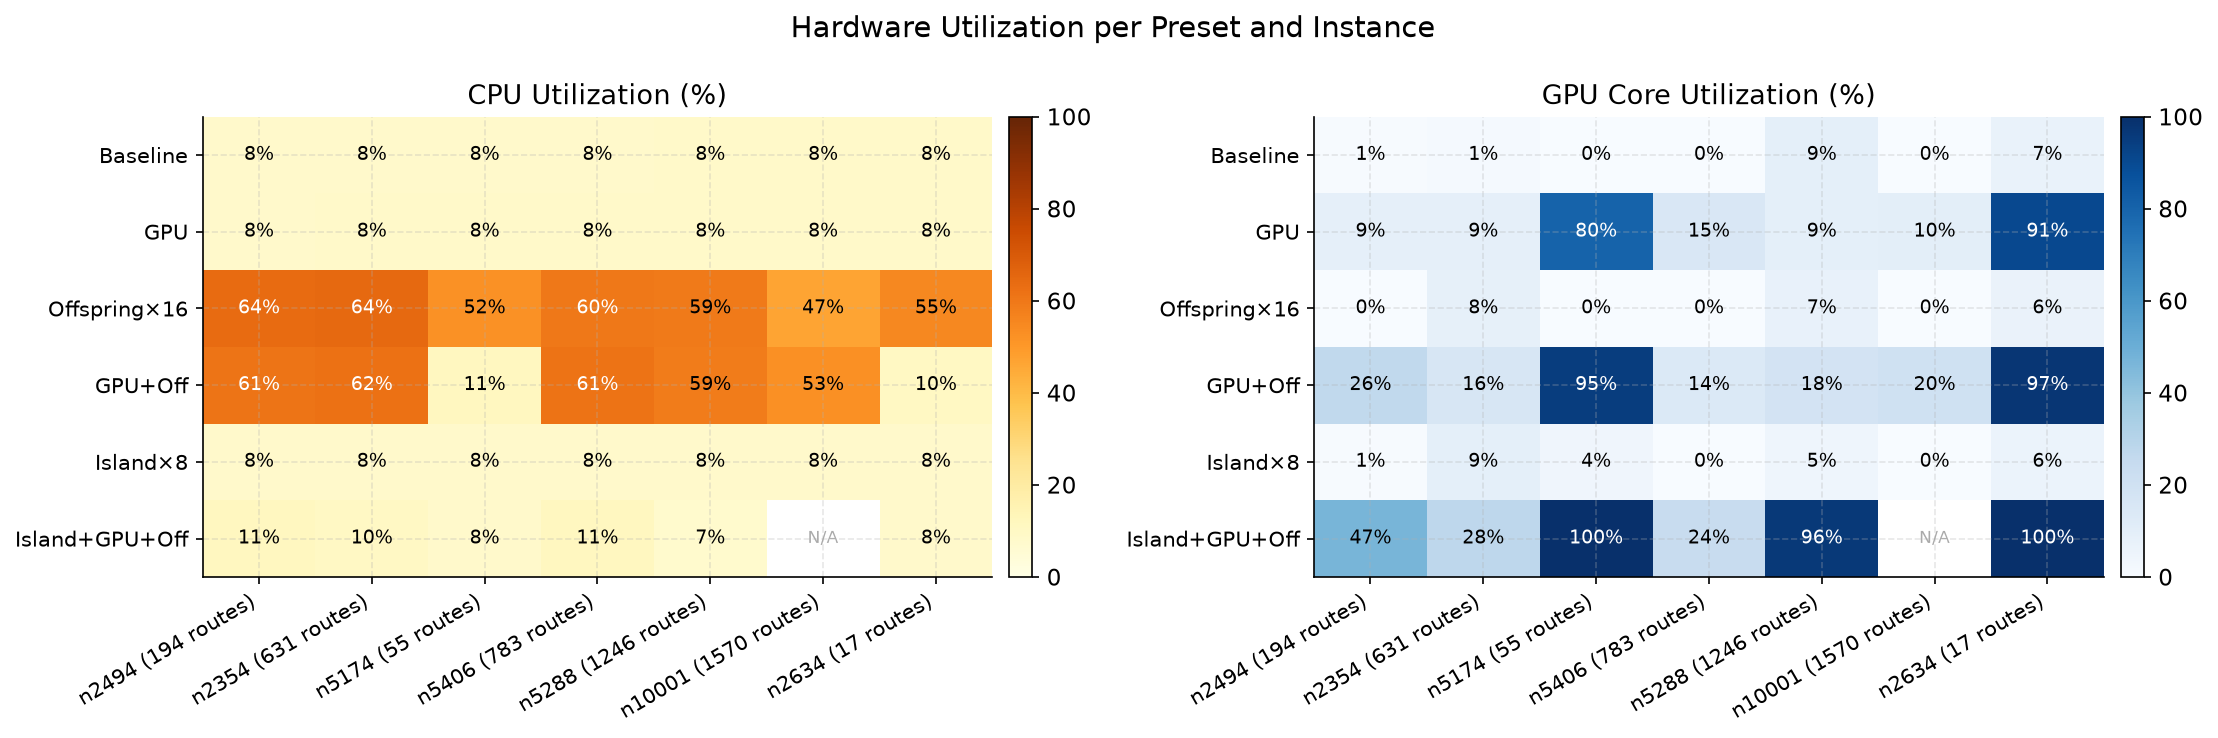
\includegraphics[width=\textwidth,height=0.74\textheight,keepaspectratio]{03_hw_utilization_heatmap.png}
\end{frame}

\begin{frame}{Dlaczego GPU ożywa przy małej liczbie pojazdów?}
  \begin{columns}[T]
    \begin{column}{0.56\textwidth}
      Karta jest wydajna tylko wtedy, gdy ma \textbf{dużo równoległej pracy na jedno wywołanie}.
      \vspace{0.4em}
      \begin{itemize}
        \item SWAP* porównuje \textbf{pary klientów} wewnątrz i między trasami — liczba par rośnie z \textbf{kwadratem długości trasy}.
        \item \textbf{Mało pojazdów} $\Rightarrow$ trasy bardzo \textbf{długie} (nawet $\sim$155 klientów/trasę) $\Rightarrow$ ogromne, gęste bloki pracy $\Rightarrow$ \good{rdzenie GPU zajęte}.
        \item \textbf{Dużo pojazdów} $\Rightarrow$ trasy \textbf{malutkie} (3--4 klientów) $\Rightarrow$ pracy jak na lekarstwo $\Rightarrow$ dominuje narzut uruchomienia kernela i transferu $\Rightarrow$ \bad{GPU głoduje}.
      \end{itemize}
    \end{column}
    \begin{column}{0.44\textwidth}
      \centering
      \scriptsize
      \begin{tabular}{l r r}
        \toprule
        Instancja & \makecell{klienci\\/trasę} & \makecell{rdzenie\\GPU} \\
        \midrule
        XL-n2634-\textbf{k17}   & 155 & \good{91\%} \\
        XL-n5174-\textbf{k55}   & 94  & \good{80\%} \\
        XL-n2494-k194           & 13  & 9\% \\
        XL-n5406-k783           & 7   & 15\% \\
        XL-n5288-k1246          & 4   & 9\% \\
        XL-n2354-k631           & 4   & 9\% \\
        \bottomrule
      \end{tabular}
      \par\vspace{0.4em}
      {\tiny ,,k'' w nazwie = liczba pojazdów. Średnia długość trasy $=n/k$.}
    \end{column}
  \end{columns}
\end{frame}


% ===========================================================================
\section{Spojrzenie biznesowe}
% ===========================================================================
\begin{frame}{Czy to się opłaca? Bilans kosztów i korzyści}
  \begin{columns}[T]
    \begin{column}{0.5\textwidth}
      \textbf{Korzyść}
      \begin{itemize}
        \item poprawa jakości: \good{$<1\%$} (mediana), niestabilna,
        \item czasem \bad{pogorszenie} jakości.
      \end{itemize}
    \end{column}
    \begin{column}{0.5\textwidth}
      \textbf{Koszt}
      \begin{itemize}
        \item karta GPU (capex) + 8 rdzeni CPU + środowisko MPI,
        \item ~3$\times$ większa złożoność kodu (CUDA + OpenMP + MPI),
        \item utrzymanie, debugowanie, sprzęt.
      \end{itemize}
    \end{column}
  \end{columns}
  \vfill
  \begin{alert}{Wniosek biznesowy}
    Płacimy znaczną cenę sprzętową i inżynierską za zysk jakości na poziomie szumu. \textbf{Stosunek koszt/korzyść jest niekorzystny.}
  \end{alert}
\end{frame}

\begin{frame}{Zużycie energii — perspektywa ,,perf-per-watt''}
  Szacunek poglądowy (rzędy wielkości, ten sam czas 600 s):
  \vfill
  \centering
  \small
  \begin{tabular}{l c c c}
    \toprule
    Wariant & Pobór mocy & Energia (600 s) & Zysk jakości \\
    \midrule
    Baseline (1 rdzeń)        & ~50 W            & ~8 Wh   & --- \\
    Offspring (8 rdzeni)      & ~130 W           & ~22 Wh  & \good{$\sim$+1\%} \\
    GPU + offspring           & ~280 W           & ~47 Wh  & \good{$\sim$+0,5\%} \\
    Wyspy + GPU + offspring   & ~300 W           & ~50 Wh  & \bad{często $<0$} \\
    \bottomrule
  \end{tabular}
  \vfill
  \footnotesize Pobór mocy mierzony za pomocą urządzenia monitorującego pobór mocy z gniazdka. Wartości uśrednione dla różnych instancji. 
\end{frame}


% ===========================================================================
\section{Wnioski}
% ===========================================================================
\begin{frame}{Wnioski}
  Niestety nasze podejście do problemu było wadliwe od samego początku — próbowaliśmy \textbf{dopasować algorytm do równoległości}, 
  zamiast \textbf{dopasować równoległość do algorytmu}. HGS jest zbudowany wokół sekwencyjnej, adaptacyjnej pętli, która nie daje 
  się łatwo rozbić na niezależne kawałki. Próby zrównoleglenia tej pętli \textbf{nie poprawiły jakości} w sposób istotny, a czasem ją
  pogorszyły — bo wąskim gardłem nie jest przepustowość, lecz algorytm i struktura zależności danych.\\
  \vfill
  Lepszym podejściem byłoby zbadanie algorytmów polegających na iteracyjnym ulepszaniu rozwiązania, które są \textbf{zaprojektowane z myślą o równoległości} 
\end{frame}

\begin{frame}{Czego się nauczyliśmy?}
  \begin{itemize}
    \item Lepiej poznaliśmy mechanizmy działania algorytmów genetycznych i metaheurystycznych.
    \item Nauczyliśmy się technologii równoległych, szczególnie openMP oraz MPI, i ich zastosowania w praktyce.
    \item Chociaż nie udało się zawżeć tego w końcowym raporcie, to mieliśmy możliwość skorzystania z dużego klastra obliczeniowego
    i nauczenia się podstaw pracy z systemem kolejkowym, zarządzania zadaniami i monitorowania zasobów.
  \end{itemize}
\end{frame}


\begin{frame}{}
  \vfill
  \centering
  \Large Dziękujemy za uwagę.\\[1em]
  \vfill
\end{frame}

\end{document}

